\documentclass[]{article}
\usepackage{lmodern}
\usepackage{amssymb,amsmath}
\usepackage{ifxetex,ifluatex}
\usepackage{fixltx2e} % provides \textsubscript
\ifnum 0\ifxetex 1\fi\ifluatex 1\fi=0 % if pdftex
  \usepackage[T1]{fontenc}
  \usepackage[utf8]{inputenc}
\else % if luatex or xelatex
  \ifxetex
    \usepackage{mathspec}
  \else
    \usepackage{fontspec}
  \fi
  \defaultfontfeatures{Ligatures=TeX,Scale=MatchLowercase}
\fi
% use upquote if available, for straight quotes in verbatim environments
\IfFileExists{upquote.sty}{\usepackage{upquote}}{}
% use microtype if available
\IfFileExists{microtype.sty}{%
\usepackage{microtype}
\UseMicrotypeSet[protrusion]{basicmath} % disable protrusion for tt fonts
}{}
\usepackage[margin=1in]{geometry}
\usepackage{hyperref}
\hypersetup{unicode=true,
            pdftitle={Cross-study learning for the epigenomic prediction of cardiovascular disease risk},
            pdfborder={0 0 0},
            breaklinks=true}
\urlstyle{same}  % don't use monospace font for urls
\usepackage{graphicx,grffile}
\makeatletter
\def\maxwidth{\ifdim\Gin@nat@width>\linewidth\linewidth\else\Gin@nat@width\fi}
\def\maxheight{\ifdim\Gin@nat@height>\textheight\textheight\else\Gin@nat@height\fi}
\makeatother
% Scale images if necessary, so that they will not overflow the page
% margins by default, and it is still possible to overwrite the defaults
% using explicit options in \includegraphics[width, height, ...]{}
\setkeys{Gin}{width=\maxwidth,height=\maxheight,keepaspectratio}
\IfFileExists{parskip.sty}{%
\usepackage{parskip}
}{% else
\setlength{\parindent}{0pt}
\setlength{\parskip}{6pt plus 2pt minus 1pt}
}
\setlength{\emergencystretch}{3em}  % prevent overfull lines
\providecommand{\tightlist}{%
  \setlength{\itemsep}{0pt}\setlength{\parskip}{0pt}}
\setcounter{secnumdepth}{0}
% Redefines (sub)paragraphs to behave more like sections
\ifx\paragraph\undefined\else
\let\oldparagraph\paragraph
\renewcommand{\paragraph}[1]{\oldparagraph{#1}\mbox{}}
\fi
\ifx\subparagraph\undefined\else
\let\oldsubparagraph\subparagraph
\renewcommand{\subparagraph}[1]{\oldsubparagraph{#1}\mbox{}}
\fi

%%% Use protect on footnotes to avoid problems with footnotes in titles
\let\rmarkdownfootnote\footnote%
\def\footnote{\protect\rmarkdownfootnote}

%%% Change title format to be more compact
\usepackage{titling}

% Create subtitle command for use in maketitle
\providecommand{\subtitle}[1]{
  \posttitle{
    \begin{center}\large#1\end{center}
    }
}

\setlength{\droptitle}{-2em}

  \title{Cross-study learning for the epigenomic prediction of cardiovascular
disease risk}
    \pretitle{\vspace{\droptitle}\centering\huge}
  \posttitle{\par}
    \author{}
    \preauthor{}\postauthor{}
    \date{}
    \predate{}\postdate{}
  
\usepackage{booktabs}
\usepackage{longtable}
\usepackage{array}
\usepackage{multirow}
\usepackage{wrapfig}
\usepackage{float}
\usepackage{colortbl}
\usepackage{pdflscape}
\usepackage{tabu}
\usepackage{threeparttable}
\usepackage{threeparttablex}
\usepackage[normalem]{ulem}
\usepackage{makecell}
\usepackage{xcolor}

\begin{document}
\maketitle

\hypertarget{abstract}{%
\section{Abstract}\label{abstract}}

Epigenome-wide association studies for cardiometabolic risk factors have
discovered multiple loci associated with incident cardiovascular disease
(CVD). However, few studies have sought to directly optimize a predictor
of CVD risk. Furthermore, it is traditionally challenging to train
multivariate models across multiple studies in the presence of study- or
batch effects. Here, we analyzed existing DNA methylation data collected
using the Illumina HumanMethylation450 microarray to create a predictor
of CVD risk across three cohorts: Women's Health Initiative, Framingham
Heart Study Offspring Cohort, and Lothian Birth Cohorts. We trained Cox
proportional hazards-based elastic net regressions for incident CVD
separately in each cohort, and used a recently-introduced cross-study
learning approach to integrate these individual predictions into an
ensemble predictor. The methylation-based risk score (MRS) predicted CVD
time-to-event in a held-out fraction of the Framingham dataset (HR per
SD = 1.32, p = 2e-4) and predicted myocardial infarction status in the
independent REGICOR dataset (OR per SD = 2.2, p = 1e-6). These
associations remained after adjustment for traditional cardiovascular
risk factors, and were consistently stronger than those from elastic net
models trained on a directly merged dataset. Additionally, we
investigated interactions between the MRS and both genetic and
biochemical CVD risk, showing preliminary evidence of an enhanced
predictive power in those with less traditional risk factor elevation
and suggesting that the MRS may enable the discovery of high-risk
individuals that would be missed by alternative risk metrics.

\hypertarget{introduction}{%
\section{Introduction}\label{introduction}}

DNA methylation is an important epigenetic pathway through which genetic
variants and environmental exposures impact disease risk (Bonder et al.
2016; Tobi et al. 2018). Methylation at specific
cytosine-phosphate-guanine (CpG) sites has been associated with disease
in epigenome-wide association studies, even showing associations in
blood as a convenient but non-target tissue such as for type 2 diabetes
(Bacos et al. 2016). Methylation-based risk scores allow genome-wide
aggregation of epigenetic information, similarly to the more established
genetic risk scores, and allow for the use of models with arbitrary
complexity. These risk scores are often developed initially by using
methylation as a proxy for disease risk factors, such as BMI (Wahl et
al. 2017) and general aging-related morbidity (Levine et al. 2018).
Alternatively, given sufficient sample size, epigenetic associations
with disease risk can be modeled directly (Hao et al. 2017).

Associations between DNA methylation and cardiovascular disease (CVD)
have been explored in many different cohorts and using diverse
approaches. Cross-sectional associations have been found across multiple
relevant tissues, namely blood, aorta, and other vascular tissues
(Fernández-Sanlés et al. 2017). Some investigations aimed at
cardiovascular risk factors have discovered CpGs predictive of CVD
development (Hedman et al. 2017; Aslibekyan et al. 2018), while
Mendelian randomization approaches have suggested causality of at least
some of these CpG-risk factor associations (Richardson et al. 2017). The
few studies directly modeling incident CVD as a primary outcome have
either been conducted using only global (not locus-specific) methylation
levels (Baccarelli et al. 2010), or have found limited additional
predictive power in the presence of known risk factors (Guarrera et al.
2015). We have previously investigated methylation regions and modules
associating with incident CVD, generating mechanistic insights but
without aggregating these results into a direct predictor of risk
(Westerman et al. 2018). Additionally, it is unclear how the CVD risk
tracked by DNA methylation is redundant with or complementary to
existing risk metrics, including genetic scores (Khera et al. 2018) and
those based on traditional cardiovascular risk factors (e.g.~the
Framingham Risk Score for generalized CVD) (D'Agostino et al. 2008).

Due to the many sources of heterogeneity across population-scale
cohorts, it is beneficial to combine signal across cohorts when
performing association studies or training predictive genomic models.
Such a strategy can increase sample size while attenuating the effect of
study-specific biases and confounding factors, but can be prone to
emergent sources of confounding from ``batch'' effects or other
systematic biases in methylation data across cohorts. This is especially
problematic when there is notable class imbalance (different outcome
frequencies or distributions) across cohorts (Goh, Wang, and Wong 2017).
The most common and straightforward method for dealing with this
heterogeneity is to use meta-analysis, but standard meta-analysis
approaches are restricted to univariate (i.e.~one CpG site at a time)
models. Other approaches include batch effect correction on the input
dataset (e.g.~ComBat (Johnson, Li, and Rabinovic 2007)), direct
adjustment for batch/study in linear models, or adjustment for derived
variables intended to capture technical biases (e.g.~surrogate variable
analysisn (Leek and Storey 2007)), but these approaches can often lead
to over- or under-estimates of true biological effects (Goh, Wang, and
Wong 2017), and may be less amenable to complex or nonlinear models.
Another approach described recently, cross-study learning, uses an
alternative strategy to tackle the problem by creating an ensemble
predictor consisting of one or multiple models per cohort, all trained
to predict the same outcome (Patil and Parmigiani 2018). This strategy
allows the use of arbitrarily complex models and the contribution of
multiple training cohorts while avoiding technical confounding from
direct combination of the datasets.

In order to develop an improved DNA methylation-based cardiovascular
risk predictor using multiple training cohorts, we used a cross-study
learning method to develop an ensemble of penalized time-to-event
regression risk models. The resulting composite risk score performed
well in a held-out data subset, predicting survival even in the presence
of traditional risk factors, and surpassing the performance of models
trained on naively merged datasets. External validation was achieved in
a case-control for prevalent myocardial infarction (MI). Further,
interactions were assessed between the composite methylation-based risk
score and other risk predictors, finding no consistent relationship to a
genome-wide genetic risk score, but a potentially enhanced prediction in
those with low Framingham Risk Scores.

\hypertarget{results}{%
\section{Results}\label{results}}

\hypertarget{cross-study-learner-model-development}{%
\subsection{Cross-study learner model
development}\label{cross-study-learner-model-development}}

Epigenomic model development was performed in three cohorts, including
the Women's Health Initiative (WHI), Framingham Heart Study Offspring
Cohort (FHS), and Lothian Birth Cohorts of 1936 (LBC). The FHS dataset
was divided into two functionally separate groups (FHS-JHU and FHS-UM)
based on differences in subject selection and geographic location of
laboratory methylation analysis (see Methods). Further details of the
populations can be found in Table 1.

\begin{table}[t]

\caption{\label{tab:pop-description}Baseline parameters of the populations used for model develpment}
\centering
\begin{threeparttable}
\begin{tabular}{lllll}
\toprule
Study/Subset & WHI & FHS-JHU & LBC & FHS-UM\\
Sample size & 2023 & 484 & 818 & 2103\\
Age & 65 (59-70) & 71 (64-77) & 69 (68-70) & 64 (59-71)\\
Sex (\% female) & 100 & 30 & 50 & 60\\
\addlinespace[0em]
\multicolumn{5}{l}{Ancestry}\\
\hspace{1em}\% European & 47 & 100 & 100 & 100\\
\hspace{1em}\% African American & 32 & 0 & 0 & 0\\
\hspace{1em}\% Hispanic & 20 & 0 & 0 & 0\\
Body mass index & 29.1 (25.5-33.3) & 28.2 (25.5-31.3) & 27.5 (24.9-30.3) & 27.4 (24.3-31)\\
LDL cholesterol & 150 (126-175) & 88 (73-107) & 118 (89.5-150.3) & 107 (87-128)\\
HDL cholesterol & 51 (43-60) & 49 (40-60) & 56.1 (47.2-68.3) & 56 (45.8-69)\\
Triglycerides & 127 (92-177) & 101.5 (75-141.2) & 128.4 (97.4-171.2) & 102 (73-142)\\
Fasting glucose & 96 (88.6-108) & 106 (97-116) & Unavailable & 100 (94-109)\\
Systolic blood pressure & 131 (120-143) & 130 (117-143) & 148.7 (137-161.3) & 126 (116-138)\\
\addlinespace[0em]
\multicolumn{5}{l}{\# CVD events}\\
\hspace{1em}Prior only & 0 & 127 & 70 & 112\\
\hspace{1em}Incident only & 1009 & 67 & 133 & 146\\
\hspace{1em}Prior and incident & 0 & 58 & 164 & 34\\
\bottomrule
\end{tabular}
\begin{tablenotes}
\item * Continuous values shown as: median (interquartile range)
\item * WHI = Women's Health Initiative, FHS-JHU = Framingham Heart Study Offspring Cohort (Johns Hopkins University subset), LBC = Lothian Birth Cohorts 1936, FHS-UM = Framingham Heart Study Offspring Cohort (University of Minnesota subset)
\end{tablenotes}
\end{threeparttable}
\end{table}

Fig. 1 outlines the computational workflow. Briefly, a cross-study
learning (CSL) model was developed by training time-to-event elastic net
regressions on three of the datasets, while holding out the FHS-UM
subset for evaluation. Next, a model trained on all four datasets was
subject to external replication in the REGICOR study. CSL model CpGs
were characterized as to their potential biological function, and model
performance was assessed across strata of alternative cardiovascular
risk metrics.

The initial predictor was developed by training individual penalized Cox
proportional hazards regression models (single-study learners, or SSLs)
in each of the three training cohorts (WHI, FHS-JHU, and LBC).
Predictions from these models were aggregated through the ``stacking''
method, in which the outcomes and model predictions from each of the
individual datasets are combined, and a regression is used to assign
weights to each of the model predictions (see Methods). This procedure
led to FHS-JHU dropping out of the ensemble model, with weights for this
initial predictor as follows: 0.6 (WHI), 0.0 (FHS-JHU), and 0.4 (LBC).

\begin{figure}
\centering
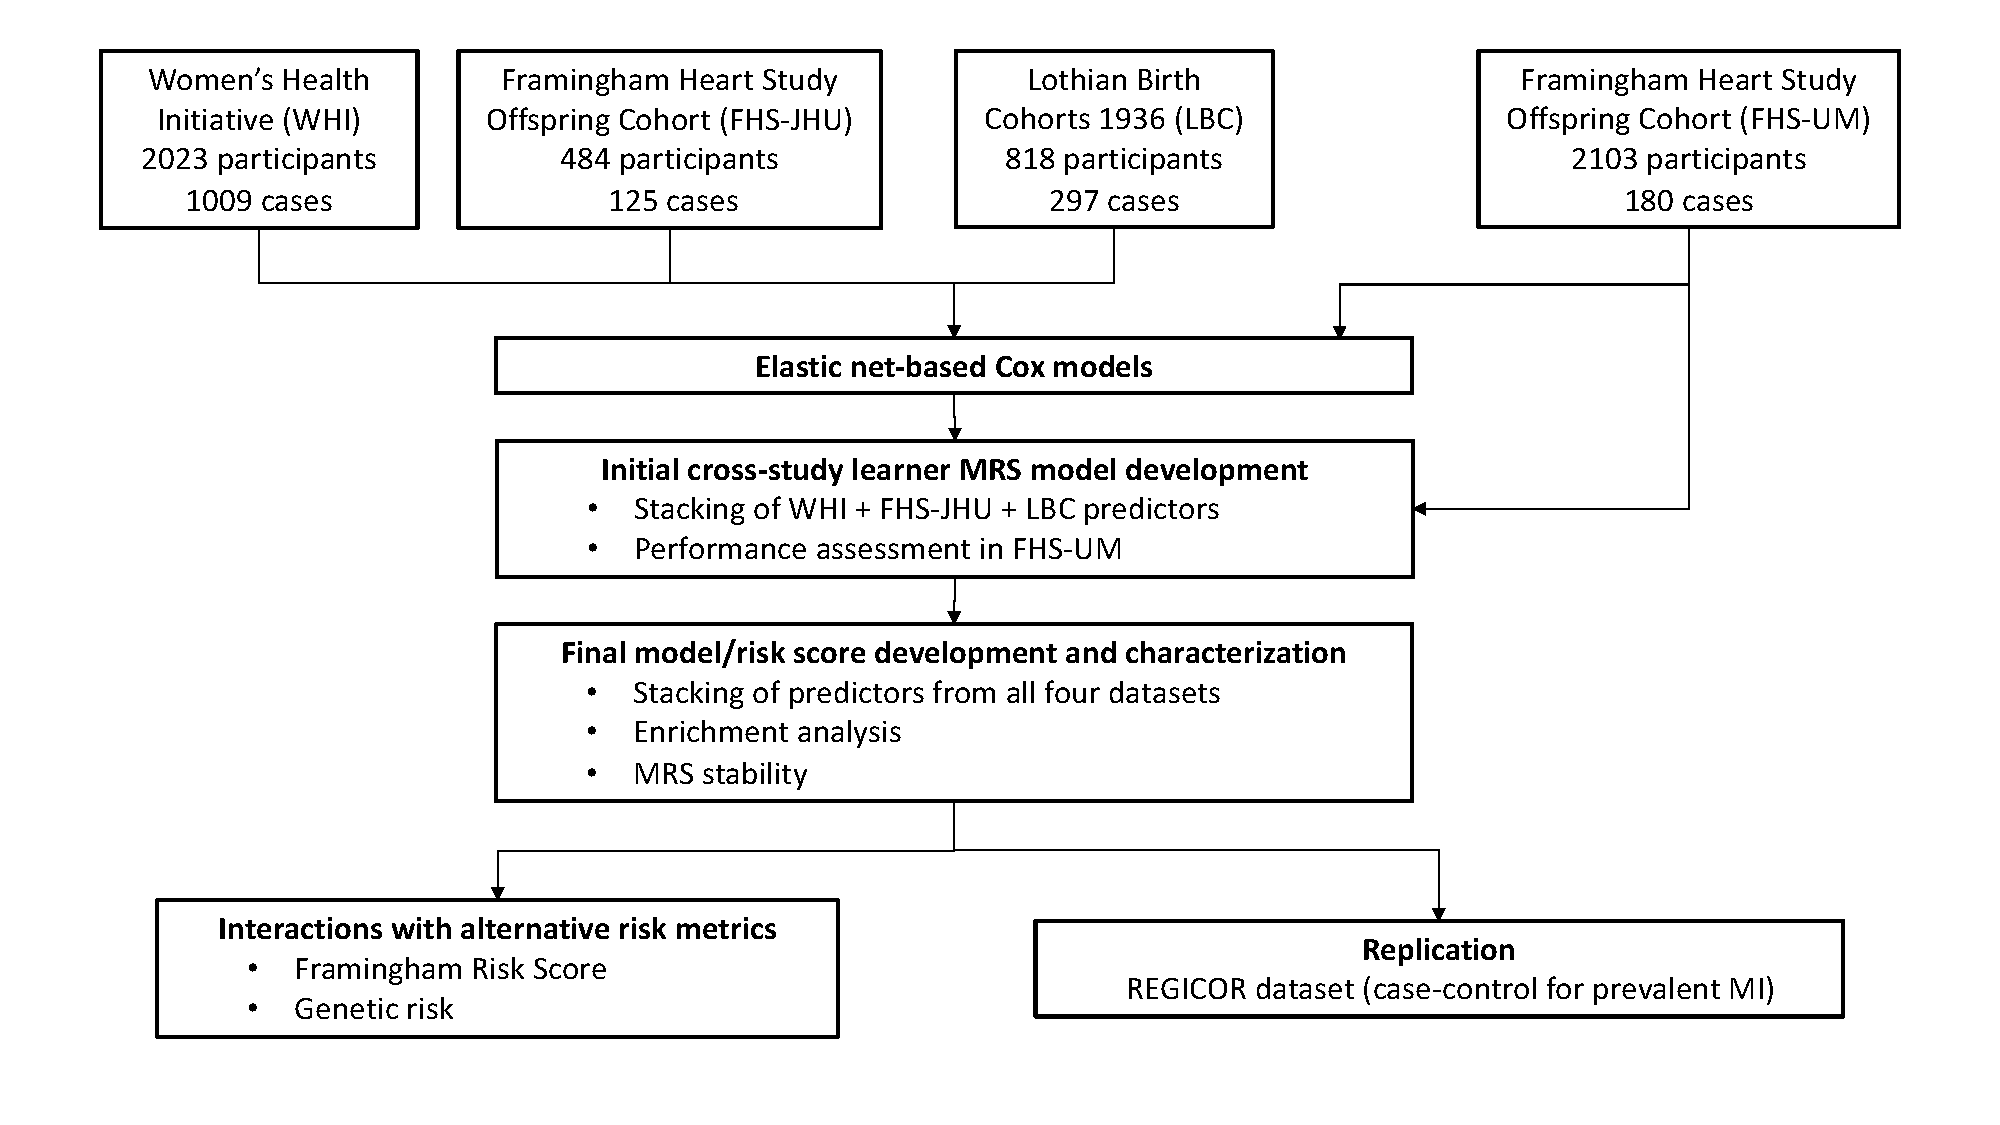
\includegraphics{workflow.pdf}
\caption{Computational workflow for MRS development and evaluation. The
initial MRS was trained in three cohorts with FHS-UM held out to
evaluate performance. The final MRS was then trained using all four
datasets and examined for biological significance, before testing for
prevalent MI discrimination in an independent cohort and assessment of
interactions with genetic and traditional risk scores.}
\end{figure}

\hypertarget{assessment-in-held-out-fhs-subset}{%
\subsection{Assessment in held-out FHS
subset}\label{assessment-in-held-out-fhs-subset}}

\begin{table}[t]

\caption{\label{tab:fhs-holdout}MRS performance in held-out FHS subset}
\centering
\begin{threeparttable}
\begin{tabular}{lrl}
\toprule
Model & HR per s.d. MRS & P-value\\
\midrule
Unadjusted\textsuperscript{1} & 1.62 & 7.5e-12\\
Basic\textsuperscript{2} & 1.32 & 2.2e-04\\
Plus risk factors\textsuperscript{3} & 1.29 & 2.2e-03\\
FRS only\textsuperscript{4} & 1.40 & 5.9e-06\\
\bottomrule
\end{tabular}
\begin{tablenotes}
\item[1] No covariates
\item[2] Adjusted for age, sex, and estimated cell type fractions
\item[3] Additionally adjusted for BMI, LDL, HDL, SBP, diabetes status, and current smoking
\item[4] Adjusted for Framingham Risk Score only
\end{tablenotes}
\end{threeparttable}
\end{table}

\begin{table}[t]

\caption{\label{tab:fhs-holdout}Comparison of Cox regression coefficient estimates between the CSL and combined model options.}
\centering
\begin{threeparttable}
\begin{tabular}{llll}
\toprule
\multicolumn{1}{c}{} & \multicolumn{3}{c}{HR per s.d. MRS} \\
\cmidrule(l{3pt}r{3pt}){2-4}
Model & Combined & ComBat & CSL\\
\midrule
Unadjusted & 1.51 [1.3-1.76] & 1.75 [1.54-1.99] & 1.62 [1.41-1.86]\\
Basic & 1.21 [1.02-1.42] & 1.39 [1.18-1.63] & 1.32 [1.14-1.54]\\
Plus risk factors & 1.12 [0.94-1.33] & 1.28 [1.07-1.53] & 1.29 [1.1-1.52]\\
FRS only & 1.39 [1.2-1.62] & 1.56 [1.36-1.78] & 1.4 [1.21-1.62]\\
\bottomrule
\end{tabular}
\begin{tablenotes}
\item * Results are presented as: OR per s.d. MRS [95\% CI]
\item * Combined model naively combines all datasets while adjusting for study, whereas ComBat adjusts the data themselves to remove variation across studies while preserving class differences.
\item * Model covariates as in Table 2
\end{tablenotes}
\end{threeparttable}
\end{table}

\begin{figure}
\centering
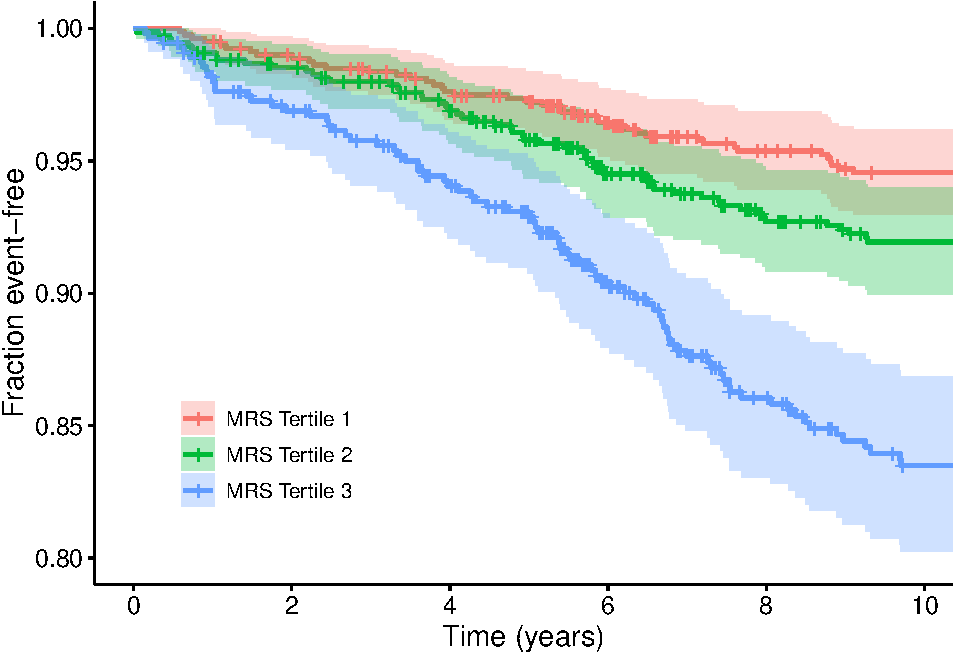
\includegraphics{figures/km-plot-1.pdf}
\caption{Kaplan-Meier survival curves in the held-out FHS-UM dataset.
Individual curves correspond to tertiles of the initial (3-dataset) MRS.
Vertical ticks correspond to censored observations, and colored bands
represent 95\% confidence intervals for tertile-specific survival
curves.}
\end{figure}

Stacking of the three initial predictors resulted in model weights of
0.6, 0, and 0.4 for WHI, FHS-JHU, and LBC, respectively (i.e.~FHS-JHU
did not ultimately contribute to the initial model). The resulting
ensemble predictor was evaluated using robust Cox proportional hazards
models in FHS-UM, showing strong associations with incident CVD in an
unadjusted model (HR=1.62, p=6.03e-14), which was attenuated partially
through adjustment for standard covariates (age, sex, and estimated cell
type fractions) as well as CVD risk factors (Table 2). These results
were robust to sensitivity analyses excluding all individuals who
experienced prior CVD events (Supp. Table S1).

When compared to the models based on naive combination of the datasets
(``Combined''), the CSL model performed consistently better across all
sets of covariates (Table 3). However, its performance was equivalent or
worse than the single model trained on a ComBat-preprocessed dataset
(note that FHS-UM was not included in the ComBat adjustment dataset so
as not to allow the procedure to inject bias).

\hypertarget{final-csl-model-characterization}{%
\subsection{Final CSL model
characterization}\label{final-csl-model-characterization}}

\begin{figure}
\centering
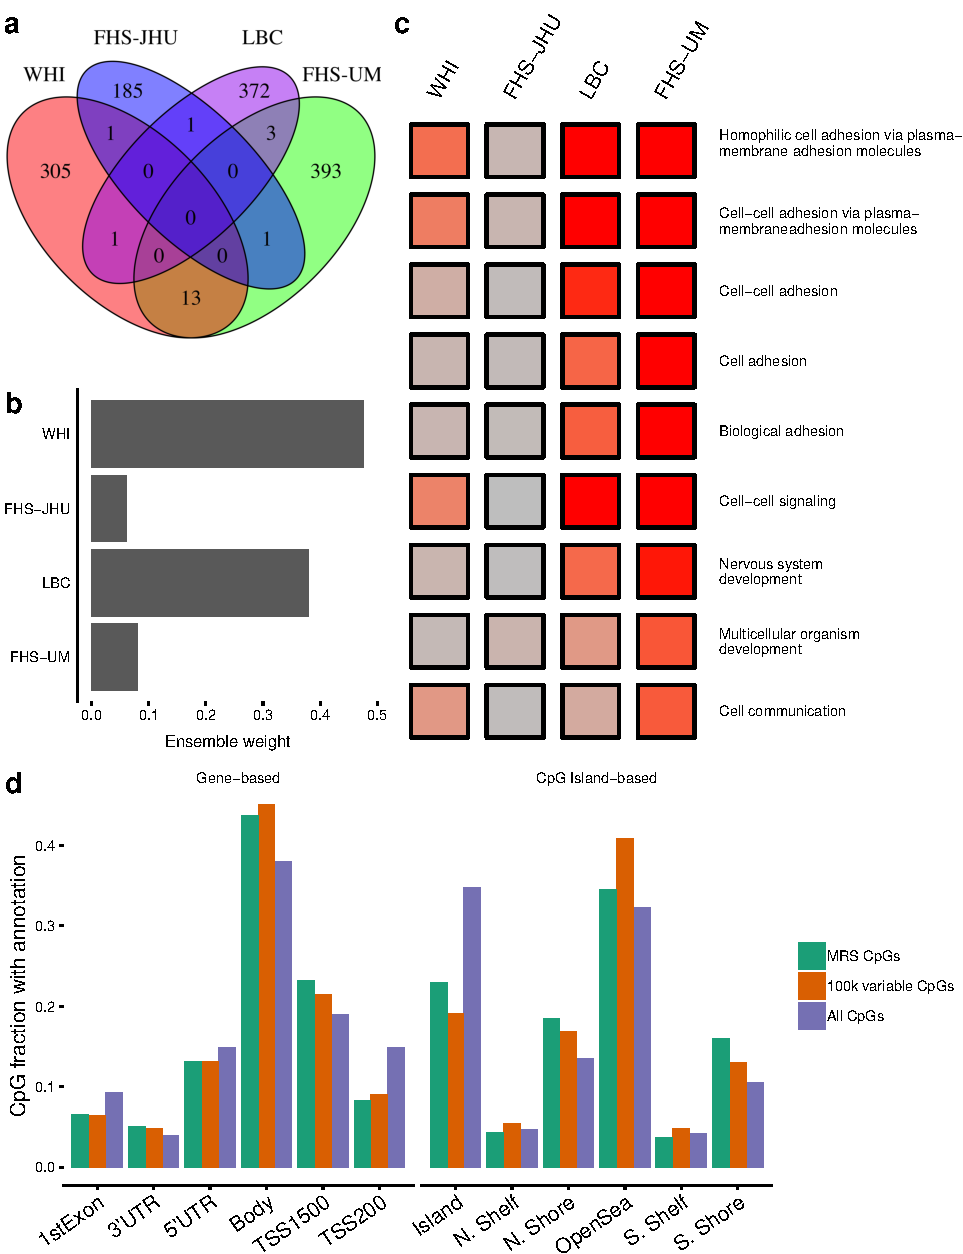
\includegraphics{figures/characterization-1.pdf}
\caption{Characterization of the final CSL model. a) Overlap of CpG
sites in the four individual predictors constituting the final model. b)
Study-specific weights for constructing the ensemble model (derived from
the ``stacking'' regression). c) Results from Gene Ontology-based
enrichment analysis using genes annotated to SSL component CpGs. All GO
terms with false discovery rate \textless{} 0.2 in any cohort are shown,
and colored according to -log(p-value) for enrichment in each SSL. d)
Proportion of CpGs in the full set of CSL CpGs (union of CpG sets in
each component SSL) compared to the 100,000 most variable CpGs (as used
in SSL model development) and the full set of available CpGs. Groupings
according to both gene-based and CpG island-based CpG annotations are
shown.}
\end{figure}

The stacking regression in the final CSL model gave the most weight to
WHI (0.43) and LBC (0.40), while retaining nonzero weights for FHS-JHU
(0.04) and FHS-UM (0.12). There was very little overlap of specific CpG
sites across cohort-specific models, with a maximum of 13 CpGs shared
between two models (WHI and FHS-UM) and no CpGs shared between three or
more models (Fig. 2a). Despite this lack of site-specific overlap, there
was broad agreement for three of the four component SSL models at the
level of enriched biological processes, with all except FHS-JHU enriched
most strongly for proximity to genes involved in homophilic cell
adhesion (Fig. 2b). MRS component CpGs tended to be found in similar
genomic loci to the overall set of variable CpGs, which tended to be
enriched in gene bodies and depleted in CpG islands compared to the full
microarray CpG set. However, MRS CpGs did show a modest enrichment in
and around CpG islands compared to the set of variable CpGs (Fig. 2d).

To gain more clarity as to potential biological mechanisms represented
by the MRS, the HOMER tool was used to calculate enrichment of
transcription factor (TF) binding motifs in the MRS component CpG sites
(union of all individual SSL sites). Though no strong enrichments were
found (all q-values \textgreater{}0.05), we note that two of the top ten
hits relate to motifs found for circadian regulatory TFs (CLOCK and
NPAS) in liver (full list of HOMER results with q \textless{}0.2 in
Supp. Table S2).

To better understand the stability of the risk score over time,
intraclass correlation coefficients (ICCs) were calculated for two sets
of grouped samples: 26 technical replicates from FHS and approximately
1000 longitudinal samples (across 3 visits, or about 6 years total) from
LBC (Supp. Table S3). The technical replicates showed an ICC of 0.81,
while the longitudinal samples showed an ICC of 0.68. As would be
expected, the ICC for samples closer in time (Waves 1 \& 2) were higher
than that for samples more distant in time (Waves 1 \& 3). Based on the
observation of imperfect stability of the MRS over time as well as the
partial attenuation its predictive power after adjustment for age, its
component CpGs (the 1298-element union of all CpGs in any of the four
individual SSL models) were examined for overlap with established
epigenetic age metrics. While no enrichment was seen for the original
cross-tissue DNAm age from Horvath (Horvath 2013), strong enrichment was
seen for the morbidity-directed PhenoAge (Levine et al. 2018) (9 of 513
CpGs; p=2.3e-5) and especially the blood-specific aging marker from
Hannum et al. (Hannum et al. 2013) (14 of 71 CpGs; p=9.4e-23). We note
that these overlaps do not constitute a major fraction of either CpG
set, but are nonetheless highly statistically significant.

\hypertarget{discrimination-in-myocardial-infarction-case-control}{%
\subsection{Discrimination in myocardial infarction
case-control}\label{discrimination-in-myocardial-infarction-case-control}}

\begin{table}[t]

\caption{\label{tab:regicor}Results from replication in REGICOR MI case-control}
\centering
\begin{tabular}{llll}
\toprule
Model & ComBat & Combined & CSL\\
\midrule
Unadjusted & 1.71 [1.31-2.23] & 1.66 [1.27-2.18] & 1.85 [1.4-2.43]\\
Basic & 2.11 [1.52-2.92] & 1.75 [1.24-2.47] & 2.23 [1.62-3.07]\\
Plus risk factors & 1.8 [1.21-2.67] & 1.36 [0.88-2.11] & 1.65 [1.12-2.44]\\
\bottomrule
\multicolumn{4}{l}{* Results are presented as: OR per s.d. MRS [95\% CI]}\\
\multicolumn{4}{l}{* Model covariates as in Table 2}\\
\multicolumn{4}{l}{* All models above are adjusted for two surrogate variable analysis (SVA) components.}\\
\end{tabular}
\end{table}

As one form of replication, the MRS was investigated for its
discriminative performance in a nested case-control for prior myocardial
infarction in the REGICOR cohort (cohort description in Supp. Table S4).
Though this dataset did not contain incident events, its matching of sex
and age allowed an evaluation free of potential confounding by these
factors. The MRS was able to discriminate cases and controls in both
unadjusted (odds ratio = 1.85, p = 1.29e-5) and, to a lesser degree,
risk factor-adjusted models (odds ratio = 1.65, p = 0.012). The improved
performance of the CSL model over the ``Combined'' MRS and its
equivalent performance to the ComBat-based MRS was also confirmed in
this dataset.

\hypertarget{interactions-with-alternate-risk-metrics}{%
\subsection{Interactions with alternate risk
metrics}\label{interactions-with-alternate-risk-metrics}}

\begin{figure}
\centering
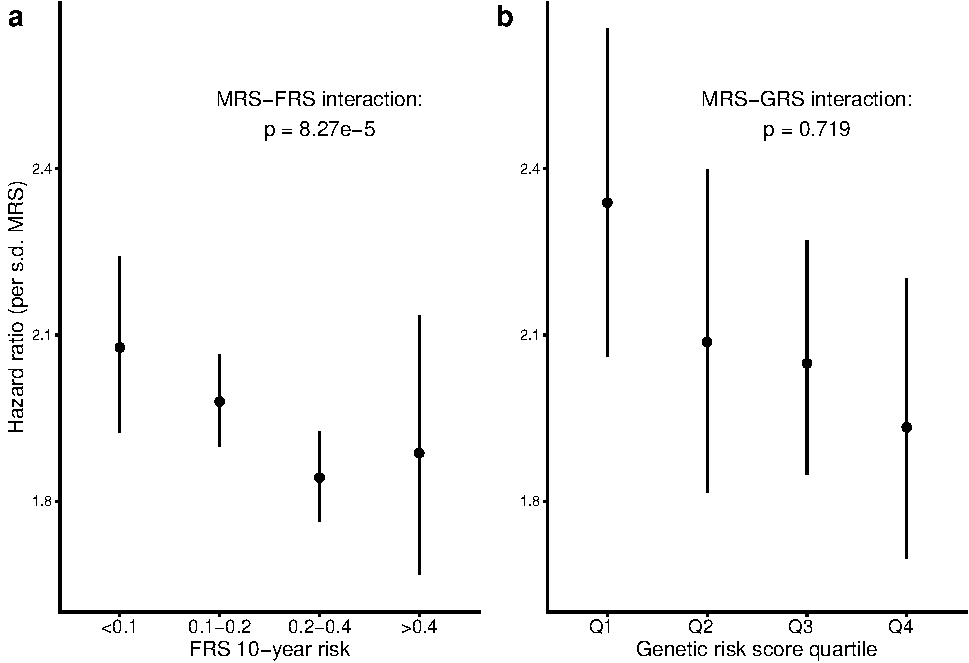
\includegraphics{figures/aggregate-interactions-1.pdf}
\caption{Interactions of MRS with other biomarkers of CVD risk. a)
Hazard ratios for the MRS within subsets of 10-year generalized CVD risk
according to the Framingham Risk Score. b) Hazard ratios for the MRS
within quartiles of a genetic cardiovascular risk score (in white
participants only). Hazard ratios are estimated using the final MRS,
which was trained using each of these datasets. Stratum-specific Cox
regressions were adjusted for age, sex, and estimated cell subtype
fractions. Error bars represent standard errors for the hazard ratio
estimates.}
\end{figure}

To understand how the present risk score interacts with other
established CVD risk metrics, the performance of the MRS was
re-evaluated after stratifying individuals by risk scores reflecting
either demographic and biochemical features (Framingham Risk Score), or
genetic variants (based on Khera et al.~2018). First, the marginal
effects of these risk scores were confirmed in each population. The
Framingham Risk Score (FRS) was strongly predictive in WHI and FHS,
while surprisingly showing no association with disease incidence in LBC
(Supp. Table S5). As the genetic score does not change over time, it was
evaluated with respect to any past or future CVD event, showing a
moderate association in WHI but no association in FHS (Supp. Table S6).

In Cox models using baseline hazards stratified by study, it appeared
that the MRS was more effective in those in lower ``traditional'' risk
strata (according to the FRS; Fig. 4). As a sensitivity analysis, the
cohorts were fully stratified into separate models, in which this
pattern was visually clear in WHI, FHS-JHU, and to some extent FHS-UM
(Supp. Fig. S1). The pattern did not appear in LBC, although we note
that the Framingham Risk Score also did not show a ``main effect'' for
predicting incident CVD in this cohort. A similar pattern appeared with
respect to genetic risk in WHI (white participants only based on the
formulation of the relevant risk score) and FHS, in which maximum MRS
performance was achieved in the lowest alternative risk stratum.
Supplementing these visual comparisons, combined Cox regressions across
all cohorts (allowing for different baseline hazards across studies)
showed a strong MRS-FRS interaction effect (12\% reduction in HR for the
MRS per 10\% increase in FRS (p = 0.000404)), while that for the MRS-GRS
interaction did not reach nominal statistical significance (0\%
reduction in HR for the MRS per standard deviation increase in GRS (p =
0.853)).

To explore the clinical potential of these interactions further, we
returned to the initial MRS (trained in 3 datasets with FHS-UM held
out). The FHS-UM dataset was filtered to include only participants with
lower CVD risk based on either FRS (\textless{}10\% estimated 10-year
risk) or GRS (lowest quartile of the GRS). Within this lower-risk
subset, participants in the upper MRS quartile had more than double the
risk of the remainder of the participants: 10\% (29/289) versus 4\%
(34/866). While a similar risk increase was observed when taking the
intersection of these low-risk groups (low FRS and low GRS), the sample
size was not enough to draw reasonable statistical conclusions (only 6
events in total).

\hypertarget{discussion}{%
\section{Discussion}\label{discussion}}

Epigenetic signatures of cardiometabolic diseases and aging in general
are being actively explored as biomarkers of disease risk that are
potentially modifiable and reveal underlying biological mechanisms.
Here, in a novel application of a cross-study ensembling method, we
introduce a DNA methylation-based score specific to cardiovascular
disease risk. The model performs better than one trained on a naive
combination of the entire dataset (though similarly to use of a batch
preprocessing algorithm), and may be most strongly predictive in
individuals predicted to be at lower risk based on traditional risk
factors.

We opted to use cross-study learning to train our risk model because we
expect that differences across cohorts (e.g.~demographic, behavioral)
may contribute to heterogeneity in both the marginal distribution of the
CpG features and the conditional distribution of the CVD outcome. Under
these conditions, the generalizability of a single-study predictor is
often obscured or overstated (Chang et al. 2015; Zhang et al. 2018).
Using the CSL, we observed improved performance in test sets as compared
to the naïve strategy of combining cohorts and training a single-study
model. This suggests that up- and down-weighting single-study models
offers an advantage compared to the increased combined sample size of
the cohort-merging strategy.

Notably, the performance of the CSL model was similar to that of the
model trained on the merged cohorts after batch adjustment via ComBat.
This suggests that the assumptions regarding heterogeneity in the
marginal distributions of the model covariates made by the ComBat
hierarchical model are met. Any heterogeneity structure that can be
captured by variation in the marginal effects can be accounted for and
removed by ComBat (Johnson, Li, and Rabinovic 2007). In practice, this
underlying structure is unknown, and we highlight that the CSL makes no
specific assumptions and was able to produce similar gains in predictive
accuracy in both the held-out FHS-UM and independent REGICOR datasets.

In assessing the stability of the MRS, we observed reasonable
reproducibility between technical replicates (ICC=0.81). ICCs for LBC
subjects over time were somewhat lower (ICC=0.68), which is to be
expected due to not only changes in environment, but also the known
epigenetic evolution with age that we observed to be enriched in the
components of our score. These ICC values suggest an imperfect but
usable reproducibility of the MRS, and an aggregate marker that is
fairly robust considering the low replicability that has been observed
for individual sites in technical replicates (general median ICC of 0.3
and mode of 0.75 in a ``high reliability'' cluster) (Bose et al. 2014).

The enrichment of the MRS component CpGs for proximity to genes related
to cell-cell adhesion (in all subsets except FHS-JHU) suggests one of
the biological patterns it tracks. As we have previously observed in a
subset of these datasets (Westerman et al. 2018), it appears that immune
activation is central to the prognostic information contained in
leukocyte DNA methylation. For example, epigenetic processes have been
shown to be involved in the activation and increased adhesion of
monocytes in response to environmental insults and metabolic stress,
though these have been explored primarily in relation to histone
modifications (Short et al. 2017). Our results provide preliminary
support for an attractive model in which a methylation-based score could
act as a monitor of cumulative stress in leukocytes and their
corresponding activation towards a more atherogenic state.

Existing epigenetic scores have shown varying strength in predicting
incident cardiovascular disease. An early investigation examined
blood-based methylation in LINE-1 elements, finding strong associations
of global hypomethylation with prevalent and incident ischemic heart
disease global (LINE-1), though additional reports showed opposite
associations of methylation at repetitive elements with CVD (Kim et al.
2010). Guarrerra et al.~developed a biomarker for MI based on global
LINE-1 and ZBTB12 gene methylation that provided a modest net
reclassification index improvement (0.23-0.47) compared to traditional
risk factors only. Multiple epigenetic aging metrics, though not
developed specifically for CVD, have been shown to predict incident CHD,
including PhenoAge (odds ratios from 1.02 to 1.08) and GrimAge (hazard
ratio = 1.07, adjusted for age and technical factors) (Levine et al.
2018; Lu et al. 2019). While these associations are statistically
significant, they do not represent clinically meaningful improvements in
discrimination. Our observed hazard ratio of 1.32 (in the held-out
FHS-UM dataset) suggests a biomarker that may be closer to clinical
relevance. We note that our component CpG sites overlap strongly with
those of these established epigenetic metrics including PhenoAge,
suggesting that it captures some of the same biological patterns.
However, the biological significance of the specific methylation changes
observed in these aging- and morbidity-related metrics, whether as
markers of failure in epigenetic regulation breakdown versus the work
down by an ``epigenetic maintenance system'' is still unclear (Horvath
2013; Lund et al. 2019).

In examining the potential clinical utility of an epigenetic risk score
for CVD, it is important to understand to what extent it is redundant or
complementary to existing risk metrics. We did not identify any robust
patterns of differential MRS performance in strata based on a recent
genetic cardiovascular risk score, meaning that individuals cannot be
prioritized for measurement of this score purely based on germline
genetic variants. There may have been lower power to detect any such
patterns from the outset, since the GRS performed only modestly in WHI
and had no discriminative power in FHS. However, we saw a pattern of
improved risk prediction in individuals whose cardiovascular risk based
on traditional metrics (here, the Framingham Risk Score) was low. While
this association is only preliminary and does not follow in one of the
four datasets examined here, it suggests that an epigenetic risk score
could help identify higher-risk individuals who otherwise would not have
been detected.

Multiple limitations should be acknowledged. While lymphocytes are known
to be important in CVD pathogenesis, there is likely additional
biological signal in other CVD-relevant tissues not examined here.
Additionally, the present definition of CVD was chosen to balance
specificity of CVD subtypes with sample size, but this balance could be
altered to focus on more specific disease subtypes (e.g.~myocardial
infarction) or a broader definition of CVD (e.g.~including heart
failure).

In sum, we have developed an epigenetic risk score for cardiovascular
disease that provides additional predictive power beyond existing risk
measures, and may show improved performance in populations otherwise
designated as low-risk. Furthermore, we have shown a novel application
of a cross-cohort ensembling method that may provide significant value
to future investigations in genomic epidemiology.

\hypertarget{methods}{%
\section{Methods}\label{methods}}

\hypertarget{study-participants-and-phenotype-collection}{%
\subsection{Study participants and phenotype
collection}\label{study-participants-and-phenotype-collection}}

WHI methylation data came from a combined case-control and pseudo
case-cohort sampling of 2129 women from the Women's Health Initiative
study, a larger prospective cohort beginning in 1993 that included over
160,000 postmenopausal women from across the United States (Anderson et
al. 1998). Included subjects had no self-reported CVD at baseline, and
cases were chosen based on incident centrally adjudicated angina,
revascularization, or CHD event during follow-up. Inclusion criteria for
methylation measurement resulted in an oversampling of African American
and Hispanic participants. Blood samples used for measurement of DNA
methylation and clinical biochemistry were taken at Exam 1. Data are
available in the dbGaP public repository (accession: phs000200.v11.p3;
downloaded on September 27, 2017).

FHS methylation data came from a substudy of the Framingham Heart Study
that measured DNA methylation in 2726 subjects from the Offspring
Cohort. The Framingham Offspring Cohort was originally established in
1971 to follow 5209 children of the original Framingham Heart Study
participants and their spouses (Kannel et al. 1979). Fasting blood
samples for both methylation and clinical biochemistry were collected
from participants at Exam 8, which took place from 2005-8. Blood samples
were also provided for clinical biochemistry measurements in previous
exams, constituting the ``past exposures'' examined here. Data are
available in the dbGaP public repository (accession: phs000007.v29.p10;
downloaded on September 27, 2017). Adjudicated cardiovascular event data
was collected through 2015, and events were defined here as any of:
myocardial infarction, angina pectoris, stroke (approximately 90\% being
ischemic), or death from CHD (Framingham event codes 1-29). FHS
methylation data were collected in two primary batches in two centers --
one in subjects from a nested case-control for CVD measured at Johns
Hopkins University (FHS-JHU) (Joehanes et al. 2013), and the other in a
larger set of remaining Framingham Offspring participants measured at
the University of Minnesota (FHS-UM).

Blood-based biochemical markers (total cholesterol, LDL, HDL,
triglycerides, glucose, hsCRP, and systolic blood pressure) were
log10-transformed for all analyses. In addition, median imputation was
used to fill missing values for BMI (20 individuals in total),
medication use, and smoking status (thus assuming no medication use and
no smoking where these values were missing). Diabetes was defined as
either use of diabetes medication or a measured fasting blood glucose
level of \textgreater{}125 mg/dL. While directly available in WHI,
pack-years of smoking was approximated in FHS by multiplying either the
number of years since starting smoking by the current number of packs
per day, or else by multiplying the number of years smoked by the median
number of packs per day (15) for those who had quit. Framingham Risk
Scores were calculated as described previously (D'Agostino et al. 2008).

The Lothian Birth Cohorts consist of two birth cohorts (born in 1921 and
1936) established in the Lothian region of Scotland (Deary et al. 2012).
Only the 1936 cohort is analyzed here. Blood samples were collected in
three waves starting in 2004, with our primary analyses here focusing on
only those samples from Wave 1 (2004-2007). LBC data are accessible
through the European Genome-phenome Archive (accession:
EGAS00001000910).

The REGICOR dataset analyzed here consisted of a nested case-control for
myocardial infarction within the larger REGICOR (REgistre GIroní del
COR) cohort from the Girona Province in Catalonia (Spain). Whole blood
samples were collected from 391 total participants, with those from
cases generally collected within 24 hours of the event. Characteristics
for this population are available in Supp. Table S4.

\hypertarget{dna-methylation-data-processing}{%
\subsection{DNA methylation data
processing}\label{dna-methylation-data-processing}}

DNA methylation data for all initial cohorts (WHI, FHS, and LBC) were
collected using the Illumina HumanMethylation450 microarray platform
(Bibikova et al. 2011) and downloaded as raw intensity files.
Preprocessing was performed using the \emph{minfi} and \emph{wateRmelon}
packages for R (Aryee et al. 2014; Pidsley et al. 2013). Sample-wise
filters were as follows: robust overall signal in the main cluster based
on visual inspection of an intensity plot, less than 10\% of probes
undetected at a detection threshold of p\textless{}1e-16, and a reported
sex matching methylation-based sex prediction. Probes were removed using
the following criteria: more than 10\% of samples undetected at a
detection threshold of p\textless{}1e-16, location in the X or Y
chromosomes, non-CpG probes, cross-hybridizing probes, probes measuring
SNPs, and probes with an annotated SNP at the CpG site or in the
single-base extension region. Samples were normalized using the Noob
method for background correction and dye-bias normalization, followed by
the BMIQ method for probe type correction (Fortin, Triche, and Hansen
2016; Teschendorff et al. 2013). Blood cell fractions for 6 blood cell
types (CD4+ T-cells, CD8+ T-cells, B-cells, natural killer cells,
monocytes, and granulocytes) were estimated using a common
reference-based method (Houseman et al. 2012), and 5 of these (excluding
granulocytes) were included in cell count-adjusted statistical models.
After quality control and filtering steps, 390597 CpG sites were shared
between the 3 datasets, formatted as beta values (ratio of methylated
signal to total microarray signal).

DNA methylation data for the REGICOR cohort were collected using the
Illumina MethylationEPIC microarray platform (Pidsley et al. 2016) and
analyzed using the \emph{wateRmelon} (Pidsley et al. 2013) and methylumi
(Davis et al. 2019) R packages. Samples were excluded based on detection
p-value \textgreater{}0.05 in at least 1\% of probes or failure to
cluster in the appropriate sex based on X chromosome methylation. Probes
were excluded based on detection p-value \textgreater{}0.05 in at least
1\% of samples, a bead count \textless{}3 in at least 5\% of samples,
discarding by Illumina based on underperformance (n=1,031) or changes in
the manufacturing process (n=977), non-CpG targets, and
cross-hybridization (n=43,979). A batch normalization was performed by
standardizing beta values to mean zero and unit variance within each
bisulfite conversion batch prior to analysis. After quality control and
preprocessing, 811,610 CpG sites across 391 individuals were available
for analysis. Participants were further excluded from analysis due to
unknown smoking habits (n=10) and unavailable information regarding
diabetes, hypertension, or hyperlipidemia (n=53). Surrogate variable
analysis (Leek and Storey 2007) was used to calculate two surrogate
variables, representing potential technical and biological confounders,
for adjustment in MRS replication models.

\hypertarget{cvd-risk-prediction-modeling}{%
\subsection{CVD risk prediction
modeling}\label{cvd-risk-prediction-modeling}}

Study-specific CVD risk prediction models were trained using penalized
Cox proportional hazards regressions with the elastic net penalty. CVD
events were defined as above, and times were right-censored based on the
most recent exam available in each cohort. The elastic alpha parameter
was set at 0.05, based on prior observations of good performance on
Illumina methylation microarray datasets (Zhuang, Widschwendter, and
Teschendorff 2012), and the penalty parameter \(\lambda\) was optimized
through 5-fold cross-validation. For each model, only the most variable
100,000 CpGs according to median absolute deviation
(\textasciitilde{}25\% of all available sites shared across platforms)
were included in order to decrease the computational burden and ensure
that the selected CpGs would have meaningful interindividual variation.

The cross-study learner (CSL) was constructed as an ensemble of
study-specific regression models. Predictions from each single-study
learner (SSL) were combined using the ``stacking'' approach (Patil and
Parmigiani 2018), implemented as follows. First, predictions from each
SSL to both itself and the other training datasets were combined into a
design matrix (with dimensions \(N_{total}\) x \# SSLs). This formed the
input to an additional penalized Cox regression (ridge regression with
\(\lambda\) optimized through 5-fold CV and coefficients restricted to
be non-negative) of all training studies at once. Coefficients from this
regression, corresponding to input study-specific SSLs, were normalized
to sum to one to produce the CSL weights. For prediction in new
datasets, SSL predictions were each standardized to mean zero and unit
variance before calculating their weighted sum (using the ``stacking''
weights) as the final CSL score.

A series of approaches for combining information across cohorts were
tested as alternatives to the CSL. The naive ``combined'' approach
consisted of simply aggregating observations from all training sets into
a single dataset and training an elastic net regression as described
above while adjusting for study as a fixed effect. The ComBat method
trained across all studies as with the ``combined'' approach, but
included an empirical Bayes-based preprocessing step to directly adjust
the dataset for study differences while preserving variation along the
``axis'' of incident CVD events (Johnson, Li, and Rabinovic 2007).

MRS evaluation in FHS was performed using Cox proportional hazards
models, with a series of models adjusting for covariates including
demographics, anthropometrics, biochemical values, and cell subtype
estimates. Robust standard errors (also known as the Huber-White
sandwich estimator) were used to account for family structure as has
been suggested for clustered data (Rogers 1993) and used for epigenetic
risk models in FHS (Lu et al. 2019). MRS evaluation in the REGICOR
case-control used logistic regression models, adjusting for the same
sets of covariates where possible, though traditional biochemical risk
factors were only available in discrete low vs.~high categories.

\hypertarget{genomic-risk-score-calculation}{%
\subsection{Genomic risk score
calculation}\label{genomic-risk-score-calculation}}

Imputed genotype data were retrieved from dbGaP (accession:
phs000746.v2.p3 (WHI) and phs000342.v18.p11 (FHS)). Variants were
filtered for imputation R-squared \textgreater{} 0.3, and annotated with
rsIDs, loci, and allelic information using the 1000 Genomes Phase 3
download from dbSNP (download date: April 13, 2018). Weights for the
genetic risk score calculation were based on the genome-wide CVD score
developed by Khera et al (Khera et al. 2018). We note that these scores
were developed only for populations of European descent, and thus are
not optimized for the mixed-ancestry WHI population. GRS were then
calculated as the weighted sum of allelic dosages, normalized by the
number of relevant SNPs available. Genotype data processing and GRS
calculation were performed using PLINK 2.0.

\hypertarget{risk-score-interaction-analysis}{%
\subsection{Risk score interaction
analysis}\label{risk-score-interaction-analysis}}

Interaction analysis was performed using similar Cox regression models
to those above, adjusting for the ``basic'' set of covariates (age, sex,
and estimated blood cell type fractions) and using robust standard error
estimates. To facilitate visual comparisons, main-effect regressions for
the MRS were fitted within risk strata defined by the FRS or GRS
separately in each dataset. To obtain overall interaction effect
estimates, an interaction between MRS and either FRS or GRS was
introduced into a combined regression including all datasets, while
allowing stratified baseline hazards (strata() argument to the coxph
function). We note that all interaction analyses were performed using
the final MRS in the same group of datasets used to train the MRS model,
meaning that the main-effect estimates were biased upwards. All
regressions assessing the GRS excluded non-white participants, based on
the fact that the polygenic CVD score was developed in individuals of
European ancestry (Khera et al. 2018).

\hypertarget{references}{%
\section*{References}\label{references}}
\addcontentsline{toc}{section}{References}

\hypertarget{refs}{}
\leavevmode\hypertarget{ref-Anderson1998}{}%
Anderson, Garnet L, Steven R Cummings, Laurence S Freedman, Curt
Furberg, Maureen M Henderson, Susan R Johnson, Lewis H Kuller, et al.
1998. ``Design of the Women's Health Initiative Clinical Trial and
Observational Study.'' \emph{Controlled Clinical Trials} 19 (1):
61--109. \url{https://doi.org/10.1016/S0197-2456(97)00078-0}.

\leavevmode\hypertarget{ref-Aryee2014}{}%
Aryee, Martin J., Andrew E. Jaffe, Hector Corrada-Bravo, Christine
Ladd-Acosta, Andrew P. Feinberg, Kasper D. Hansen, and Rafael A.
Irizarry. 2014. ``Minfi: A flexible and comprehensive Bioconductor
package for the analysis of Infinium DNA methylation microarrays.''
\emph{Bioinformatics} 30 (10). Oxford University Press: 1363--9.
\url{https://doi.org/10.1093/bioinformatics/btu049}.

\leavevmode\hypertarget{ref-Aslibekyan2018}{}%
Aslibekyan, Stella, Golareh Agha, Elena Colicino, Anh N. Do, Jari Lahti,
Symen Ligthart, Riccardo E. Marioni, et al. 2018. ``Association of
Methylation Signals With Incident Coronary Heart Disease in an
Epigenome-Wide Assessment of Circulating Tumor Necrosis Factor
\(\alpha\).'' \emph{JAMA Cardiology} 3 (6): 463--72.
\url{https://doi.org/10.1001/JAMACARDIO.2018.0510}.

\leavevmode\hypertarget{ref-Baccarelli2010}{}%
Baccarelli, A, R Wright, V Bollati, A Litonjua, A Zanobetti, L
Tarantini, D Sparrow, P Vokonas, and J Schwartz. 2010. ``Ischemic heart
disease and stroke in relation to blood DNA methylation.''
\emph{Epidemiology} 21 (6): 819--28.
\url{https://doi.org/10.1097/EDE.0b013e3181f20457}.

\leavevmode\hypertarget{ref-Bacos2016}{}%
Bacos, Karl, Linn Gillberg, Petr Volkov, Anders H Olsson, Torben Hansen,
Oluf Pedersen, Anette Prior Gjesing, et al. 2016. ``Blood-based
biomarkers of age-associated epigenetic changes in human islets
associate with insulin secretion and diabetes.'' \emph{Nature
Communications} 7. Nature Publishing Group: 11089.
\url{https://doi.org/10.1038/ncomms11089}.

\leavevmode\hypertarget{ref-Bibikova2011}{}%
Bibikova, Marina, Bret Barnes, Chan Tsan, Vincent Ho, Brandy Klotzle,
Jennie M. Le, David Delano, et al. 2011. ``High density DNA methylation
array with single CpG site resolution.'' \emph{Genomics} 98 (4):
288--95. \url{https://doi.org/10.1016/j.ygeno.2011.07.007}.

\leavevmode\hypertarget{ref-Bonder2016}{}%
Bonder, Marc Jan, René Luijk, Daria V Zhernakova, Matthijs Moed, Patrick
Deelen, Martijn Vermaat, Maarten van Iterson, et al. 2016. ``Disease
variants alter transcription factor levels and methylation of their
binding sites.'' \emph{Nature Genetics} 49 (1): 131--38.
\url{https://doi.org/10.1038/ng.3721}.

\leavevmode\hypertarget{ref-Bose2014}{}%
Bose, Maitreyee, Chong Wu, James S. Pankow, Ellen W. Demerath, Jan
Bressler, Myriam Fornage, Megan L. Grove, et al. 2014. ``Evaluation of
microarray-based DNA methylation measurement using technical replicates:
The atherosclerosis risk in communities (ARIC) study.'' \emph{BMC
Bioinformatics}. \url{https://doi.org/10.1186/1471-2105-15-312}.

\leavevmode\hypertarget{ref-Chang2015}{}%
Chang, Christopher C., Carson C. Chow, Laurent C.A.M. Tellier, Shashaank
Vattikuti, Shaun M. Purcell, and James J. Lee. 2015. ``Second-generation
PLINK: Rising to the challenge of larger and richer datasets.''
\emph{GigaScience}. \url{https://doi.org/10.1186/s13742-015-0047-8}.

\leavevmode\hypertarget{ref-DAgostino2008}{}%
D'Agostino, Ralph B., Ramachandran S. Vasan, Michael J. Pencina, Philip
A. Wolf, Mark Cobain, Joseph M. Massaro, and William B. Kannel. 2008.
``General cardiovascular risk profile for use in primary care: The
Framingham heart study.'' \emph{Circulation} 117 (6): 743--53.
\url{https://doi.org/10.1161/CIRCULATIONAHA.107.699579}.

\leavevmode\hypertarget{ref-Davis2019}{}%
Davis, Sean, Pan Du, Sven Bilke, Timothy Triche, and Oiz Bootwalla.
2019. ``methylumi: Handle Illumina methylation data.''
\url{https://doi.org/10.1016/j.neuroimage.2007.06.039}.

\leavevmode\hypertarget{ref-Deary2012}{}%
Deary, Ian J., Alan J. Gow, Alison Pattie, and John M. Starr. 2012.
``Cohort Profile: The Lothian Birth Cohorts of 1921 and 1936.''
\emph{International Journal of Epidemiology} 41 (6): 1576--84.
\url{https://doi.org/10.1093/ije/dyr197}.

\leavevmode\hypertarget{ref-Fernandez-Sanles2017}{}%
Fernández-Sanlés, Alba, Sergi Sayols-Baixeras, Isaac Subirana, Irene R
Degano, and Roberto Elosua. 2017. ``Association between DNA methylation
and coronary heart disease or other atherosclerotic events: A systematic
review.'' \url{https://doi.org/10.1016/j.atherosclerosis.2017.05.022}.

\leavevmode\hypertarget{ref-Fortin2016}{}%
Fortin, Jean-Philippe, Timothy J Triche, and Kasper D Hansen. 2016.
``Preprocessing, normalization and integration of the Illumina
HumanMethylationEPIC array with minfi.'' \emph{Bioinformatics} 33 (4).
Oxford University Press: btw691.
\url{https://doi.org/10.1093/bioinformatics/btw691}.

\leavevmode\hypertarget{ref-Goh2017}{}%
Goh, Wilson Wen Bin, Wei Wang, and Limsoon Wong. 2017. ``Why Batch
Effects Matter in Omics Data, and How to Avoid Them.''
\url{https://doi.org/10.1016/j.tibtech.2017.02.012}.

\leavevmode\hypertarget{ref-Guarrera2015}{}%
Guarrera, Simonetta, Giovanni Fiorito, N Charlotte Onland-Moret, Alessia
Russo, Claudia Agnoli, Alessandra Allione, Cornelia Di Gaetano, et al.
2015. ``Gene-specific DNA methylation profiles and LINE-1
hypomethylation are associated with myocardial infarction risk.''
\emph{Clinical Epigenetics} 7 (1): 133.
\url{https://doi.org/10.1186/s13148-015-0164-3}.

\leavevmode\hypertarget{ref-Hannum2013}{}%
Hannum, Gregory, Justin Guinney, Ling Zhao, Li Zhang, Guy Hughes,
Srinivas Sadda, Brandy Klotzle, et al. 2013. ``Genome-wide Methylation
Profiles Reveal Quantitative Views of Human Aging Rates.''
\emph{Molecular Cell} 49 (2): 359--67.
\url{https://doi.org/10.1016/j.molcel.2012.10.016}.

\leavevmode\hypertarget{ref-Hao2017}{}%
Hao, Xiaoke, Huiyan Luo, Michal Krawczyk, Wei Wei, Wenqiu Wang, Juan
Wang, Ken Flagg, et al. 2017. ``DNA methylation markers for diagnosis
and prognosis of common cancers.'' \emph{Proceedings of the National
Academy of Sciences}. \url{https://doi.org/10.1073/pnas.1703577114}.

\leavevmode\hypertarget{ref-Hedman2017}{}%
Hedman, Åsa K., Michael M. Mendelson, Riccardo E. Marioni, Stefan
Gustafsson, Roby Joehanes, Marguerite R. Irvin, Degui Zhi, et al. 2017.
``Epigenetic Patterns in Blood Associated With Lipid Traits Predict
Incident Coronary Heart Disease Events and Are Enriched for Results From
Genome-Wide Association Studies.'' \emph{Circulation: Cardiovascular
Genetics} 10 (1): e001487.
\url{https://doi.org/10.1161/CIRCGENETICS.116.001487}.

\leavevmode\hypertarget{ref-Horvath2013}{}%
Horvath, Steve. 2013. ``DNA methylation age of human tissues and cell
types.'' \emph{Genome Biology} 14 (10): R115.
\url{https://doi.org/10.1186/gb-2013-14-10-r115}.

\leavevmode\hypertarget{ref-Houseman2012}{}%
Houseman, Eugene Andres, William P Accomando, Devin C Koestler, Brock C
Christensen, Carmen J Marsit, Heather H Nelson, John K Wiencke, and Karl
T Kelsey. 2012. ``DNA methylation arrays as surrogate measures of cell
mixture distribution.'' \emph{BMC Bioinformatics} 13 (1): 86.
\url{https://doi.org/10.1186/1471-2105-13-86}.

\leavevmode\hypertarget{ref-Joehanes2013}{}%
Joehanes, Roby, Saixia Ying, Tianxiao Huan, Andrew D. Johnson, Nalini
Raghavachari, Richard Wang, Poching Liu, et al. 2013. ``Gene Expression
Signatures of Coronary Heart Disease.'' \emph{Arteriosclerosis,
Thrombosis, and Vascular Biology} 33 (6): 1418--26.
\url{https://doi.org/10.1161/ATVBAHA.112.301169}.

\leavevmode\hypertarget{ref-Johnson2007}{}%
Johnson, W. Evan, Cheng Li, and Ariel Rabinovic. 2007. ``Adjusting batch
effects in microarray expression data using empirical Bayes methods.''
\emph{Biostatistics} 8 (1). Oxford University Press: 118--27.
\url{https://doi.org/10.1093/biostatistics/kxj037}.

\leavevmode\hypertarget{ref-Kannel1979}{}%
Kannel, William B, Manning Feinleib, Patricia M. Mcnamara, Robert J
Garrison, and William P Castelli. 1979. ``An investigation of coronary
heart disease in families: The framingham offspring study.''
\emph{American Journal of Epidemiology} 110 (3): 281--90.
\url{https://doi.org/10.1093/oxfordjournals.aje.a112813}.

\leavevmode\hypertarget{ref-Khera2018}{}%
Khera, Amit V., Mark Chaffin, Krishna G. Aragam, Mary E. Haas, Carolina
Roselli, Seung Hoan Choi, Pradeep Natarajan, et al. 2018. ``Genome-wide
polygenic scores for common diseases identify individuals with risk
equivalent to monogenic mutations.''
\url{https://doi.org/10.1038/s41588-018-0183-z}.

\leavevmode\hypertarget{ref-Kim2010}{}%
Kim, Myungjin, Tiffany I. Long, Kazuko Arakawa, Renwei Wang, Mimi C. Yu,
and Peter W. Laird. 2010. ``DNA Methylation as a Biomarker for
Cardiovascular Disease Risk.'' Edited by Joel S. Bader. \emph{PLoS ONE}
5 (3): e9692. \url{https://doi.org/10.1371/journal.pone.0009692}.

\leavevmode\hypertarget{ref-Leek2007}{}%
Leek, Jeffrey T., and John D. Storey. 2007. ``Capturing heterogeneity in
gene expression studies by surrogate variable analysis.'' \emph{PLoS
Genetics}. \url{https://doi.org/10.1371/journal.pgen.0030161}.

\leavevmode\hypertarget{ref-Levine2018}{}%
Levine, Morgan E., Ake T. Lu, Austin Quach, Brian H. Chen, Themistocles
L. Assimes, Stefania Bandinelli, Lifang Hou, et al. 2018. ``An
epigenetic biomarker of aging for lifespan and healthspan.''
\emph{Aging} 10 (4): 573--91.
\url{https://doi.org/10.18632/aging.101414}.

\leavevmode\hypertarget{ref-Lu2019}{}%
Lu, Ake T., Austin Quach, James G. Wilson, Alex P. Reiner, Abraham Aviv,
Kenneth Raj, Lifang Hou, et al. 2019. ``DNA methylation GrimAge strongly
predicts lifespan and healthspan.'' \emph{Aging} 11 (2): 303--27.
\url{https://doi.org/10.18632/aging.101684}.

\leavevmode\hypertarget{ref-Lund2019}{}%
Lund, Jesper Beltoft, Shuxia Li, Jan Baumbach, Anne Marie Svane, Jacob
Hjelmborg, Lene Christiansen, Kaare Christensen, et al. 2019. ``DNA
methylome profiling of all-cause mortality in comparison with
age-associated methylation patterns.'' \emph{Clinical Epigenetics} 11
(1). BioMed Central: 23.
\url{https://doi.org/10.1186/s13148-019-0622-4}.

\leavevmode\hypertarget{ref-Patil2018}{}%
Patil, Prasad, and Giovanni Parmigiani. 2018. ``Training replicable
predictors in multiple studies.'' \emph{Proceedings of the National
Academy of Sciences}. \url{https://doi.org/10.1073/pnas.1708283115}.

\leavevmode\hypertarget{ref-Pidsley2013}{}%
Pidsley, Ruth, Chloe C Y Wong, Manuela Volta, Katie Lunnon, Jonathan
Mill, and Leonard C Schalkwyk. 2013. ``A data-driven approach to
preprocessing Illumina 450K methylation array data.'' \emph{BMC
Genomics} 14 (1). BioMed Central: 293.
\url{https://doi.org/10.1186/1471-2164-14-293}.

\leavevmode\hypertarget{ref-Pidsley2016}{}%
Pidsley, Ruth, Elena Zotenko, Timothy J Peters, Mitchell G Lawrence,
Gail P Risbridger, Peter Molloy, Susan Van Djik, et al. 2016. ``Critical
evaluation of the Illumina MethylationEPIC BeadChip microarray for
whole-genome DNA methylation profiling.'' \emph{Genome Biology} 17 (1):
208. \url{https://doi.org/10.1186/s13059-016-1066-1}.

\leavevmode\hypertarget{ref-Richardson2017}{}%
Richardson, Tom G, Jie Zheng, George Davey Smith, Nicholas J Timpson,
Tom R Gaunt, Caroline L Relton, and Gibran Hemani. 2017. ``Mendelian
Randomization Analysis Identifies CpG Sites as Putative Mediators for
Genetic Influences on Cardiovascular Disease Risk.'' \emph{American
Journal of Human Genetics} 101 (4): 590--602.
\url{https://doi.org/10.1016/j.ajhg.2017.09.003}.

\leavevmode\hypertarget{ref-Rogers1993}{}%
Rogers, W. H. 1993. ``Regression standard errors in clustered samples.''
\emph{Stata Technical Bulletin} 13: 19--23.

\leavevmode\hypertarget{ref-Short2017}{}%
Short, John D., Sina Tavakoli, Huynh Nga Nguyen, Ana Carrera, Chelbee
Farnen, Laura A. Cox, and Reto Asmis. 2017. ``Dyslipidemic Diet-Induced
Monocyte `Priming' and Dysfunction in Non-Human Primates Is Triggered by
Elevated Plasma Cholesterol and Accompanied by Altered Histone
Acetylation.'' \emph{Frontiers in Immunology} 8 (August). Frontiers:
958. \url{https://doi.org/10.3389/fimmu.2017.00958}.

\leavevmode\hypertarget{ref-Teschendorff2013}{}%
Teschendorff, Andrew E, Francesco Marabita, Matthias Lechner, Thomas
Bartlett, Jesper Tegner, David Gomez-Cabrero, and Stephan Beck. 2013.
``A beta-mixture quantile normalization method for correcting probe
design bias in Illumina Infinium 450 k DNA methylation data.''
\emph{Bioinformatics} 29 (2): 189--96.
\url{https://doi.org/10.1093/bioinformatics/bts680}.

\leavevmode\hypertarget{ref-Tobi2018}{}%
Tobi, Elmar W., Roderick C. Slieker, René Luijk, Koen F. Dekkers, Aryeh
D. Stein, Kate M. Xu, P. Eline Slagboom, et al. 2018. ``DNA methylation
as a mediator of the association between prenatal adversity and risk
factors for metabolic disease in adulthood.'' \emph{Science Advances}.
\url{https://doi.org/10.1126/sciadv.aao4364}.

\leavevmode\hypertarget{ref-Wahl2017}{}%
Wahl, Simone, Alexander Drong, Benjamin Lehne, Marie Loh, William R.
Scott, Sonja Kunze, Pei-Chien Tsai, et al. 2017. ``Epigenome-wide
association study of body mass index and the adverse outcomes of
adiposity.'' \emph{Nature} 541 (7635): 81--86.
\url{https://doi.org/10.1038/nature20784}.

\leavevmode\hypertarget{ref-Westerman2018}{}%
Westerman, Kenneth, Paola Sebastiani, Paul Jacques, Simin Liu, Dawn
DeMeo, and José M Ordovás. 2018. ``DNA methylation modules associate
with incident cardiovascular disease and cumulative risk factor
exposure.'' \emph{bioRxiv}, January, 471722.
\url{https://doi.org/10.1101/471722}.

\leavevmode\hypertarget{ref-Zhang2018}{}%
Zhang, Yuqing, Christoph Bernau, Giovanni Parmigiani, and Levi Waldron.
2018. ``The impact of different sources of heterogeneity on loss of
accuracy from genomic prediction models.'' \emph{Biostatistics},
September. \url{https://doi.org/10.1093/biostatistics/kxy044}.

\leavevmode\hypertarget{ref-Zhuang2012}{}%
Zhuang, Joanna, Martin Widschwendter, and Andrew E. Teschendorff. 2012.
``A comparison of feature selection and classification methods in DNA
methylation studies using the Illumina Infinium platform.'' \emph{BMC
Bioinformatics}. \url{https://doi.org/10.1186/1471-2105-13-59}.


\end{document}
